\documentclass[conference]{IEEEtran}

\usepackage[british]{babel}
\usepackage{cite}
\usepackage{graphicx}
\usepackage[hyphens]{url}
%\usepackage[pdftex]{hyperref}


% correct bad hyphenation here
%\hyphenation{op-tical net-works semi-conduc-tor}


\begin{document}
%
% paper title
% can use linebreaks \\ within to get better formatting as desired
\title{The Environmental Impacts of IT Use:\\A User-Oriented Perspective}


% author names and affiliations
% use a multiple column layout for up to three different
% affiliations
\author{\IEEEauthorblockN{Peter Cooper}
\IEEEauthorblockA{Faculty of Engineering\\
University of Bristol\\
Bristol, UK\\
Email: peter.cooper@bristol.ac.uk}
\and
\IEEEauthorblockN{Tom Crick}
\IEEEauthorblockA{Department of Computing\\
Cardiff Metropolitan University\\
Cardiff, UK\\
Email: tcrick@cardiffmet.ac.uk}
\and
\IEEEauthorblockN{Theo Tryfonas}
\IEEEauthorblockA{Faculty of Engineering\\
University of Bristol\\
Bristol, UK\\
Email: theo.tryfonas@bristol.ac.uk}}

% conference papers do not typically use \thanks and this command
% is locked out in conference mode. If really needed, such as for
% the acknowledgment of grants, issue a \IEEEoverridecommandlockouts
% after \documentclass


% use for special paper notices
%\IEEEspecialpapernotice{(Invited Paper)}


% make the title area
\maketitle


\begin{abstract}
This paper discusses the environmental impact of the use of
Information Technology, with a special focus on how individual user
behaviour affects this impact. By using a process life cycle
assessment, we are able to estimate the environmental impact of the IT
use of an individual within the UK over a one year period. By
estimating the energy and data consumption of an average user's
average use of an average device, and estimating the associated energy
usage (and thus CO$_2$ produced) of each stage in the data chain, summed
to a CO$_2$ value for embodied carbon of an average device. To enable
this, market segmentation is undertaken to determine the average user
and average use, along with market research to determine the average
device. Analysis of device performance in difference behaviours is
also undertaken.

Overall, device energy is seen to dominate; within device, desktops
dominate, both due to their high energy use for a given task, but also
their high standby power, which is the most significant point of
behaviour-driven waste. Geographical, behavioural and chronological
factors are all evaluated to be highly significant to the impact of a
user's IT use, along with a number of secondary factors discovered in
the evaluation. Finally, we review the current domain research, to
advise the secondary aims of furthering the understanding of the
factors affecting the environmental impact of IT and to recommend
practical improvements based on newly assessed factors.
\end{abstract}

% For peer review papers, you can put extra information on the cover
% page as needed:
% \ifCLASSOPTIONpeerreview
% \begin{center} \bfseries
% \end{center}
% \fi
%
% For peerreview papers, this IEEEtran command inserts a page break and
% creates the second title. It will be ignored for other modes.
%\IEEEpeerreviewmaketitle

\begin{IEEEkeywords}
ICT, Environmental Impact, Energy, Emissions, Life Cycle Assessment
\end{IEEEkeywords}


\section{Introduction}

\subsection{IT in Modern Society}

The invention and spread of IT is frequently cited as one of the most
defining characteristics of humanity in the last 100 years. Arguably,
no other development can claim to have had such a profound effect on
the lives of every individual on the planet since the first
exploitation of fossil fuels. Today, no other service or utility has
as vast reach across the global population; over five billion people
now own an IT device of some kind~\cite{arup-et-al:2011}, more than
those who have access to clean water or sanitation. Despite this
prevalence, IT use still continues to grow phenomenally; 90\% of all
digital data generated has been created in the last two
years~\cite{bbcnews:2012}. IT has demonstrated an exponential increase
in processing power since the creation of the first computers in the
19th century. Today, a single graphics card contains over 200 million
transistors and has more processing power than all the computers in
the Apollo 11 lunar lander~\cite{saran:2009}. There is little evidence
to suggest this growth will slow in the near future.

IT has come to influence the nature of everyday life for many
individuals. Entirely IT-contrived concepts such as social networks
have redefined how individuals interact with one another; digitisation
of finance networks now permits the trade of ineffable quantities of
wealth across the circumference of the world in imperceptibly quick
transfers; and the sheer might of modern supercomputers has enabled us
to better understand the makeup of ourselves and our universe.

For all the benefit IT’s great power has brought, as many negative,
unintended consequences can also be listed. These can be broken down
into social, economic and environmental categories; we have seen
priorities around technology education and digital
skills~\cite{brown-et-al-toce2014}, the focus on online
behaviour~\cite{oatley+crick:2014} and the global priorities around
cyber security~\cite{carr+crick-csss2015}, as well as the development
of smart cities~\cite{cosgrave-et-al:2014} and future transport
infrastructure~\cite{cooper-et-al-sose}, all at some level predicated
on cost-effective and sustainable IT infrastructure. Such costs beg
the question: just how sustainable is IT? A complex, and sparsely
answered question, these consequences and our reaction to them will be
one of the defining challenges of the 21st century.

\subsubsection{Environmental Impacts of IT}

Rising concerns over climate change and resource use, set amongst a
context of rapid user growth, has gained IT's environmental impact
much focus. IT has been associated with 1.3\% of the world’s total
carbon footprint and 3.9\% of global energy
use~\cite{wheeland:2011}. While modest in terms of overall impact, the
continued spread of IT brings great concern to how this may grow and
the fast technological pace of the sector offers the perception of
ease of change.

Like any product or service, IT has tangible environmental impacts
across all parts of its life cycle -- from design to its disposal
(cradle to grave). However, today’s interconnected and geographically
dispersed IT systems often make assessment of the impact of a given IT
action complex and highly open to interpretation and apportion. A
Process Lifecycle Carbon Assessment (LCA) is a common way of
holistically exploring a product’s life and logically apportioning the
environmental impacts involved.

\subsection{Definitions}

\subsubsection{IT}

We define the ``use of IT'' as the use of information technologies
that satisfies two criteria:

\begin{itemize}
\item Uses stored-program architecture, excluding a myriad of other
  electronic devices in use, as well as older forms of information
  technology (books, etc);
\item Primary function is that of the creation, processing or display
  of data; excluding electronic devices that use stored-program
  architecture only as a supplement to a different core function, such
  as cars, white goods, electrical toothbrushes, watches and bike
  computers.
\end{itemize}

We believe the vast majority of IT meeting these two criteria can be
summarised as follows:

\begin{enumerate}
\item Smartphones: A mobile phone based upon a stored-program
  architecture with a range of communication technologies (e.g. GSM, GPS,
  Bluetooth, etc).
\item Tablets: A device that is possible to be held in one’s hand but
  has no GSM connectivity.
\item Laptops: A device that weighs less than 4kg but greater
  than 1kg, and has the ability to run off batteries for a
  tangible duration.
\item Desktops: A device that has no ability to run off batteries for
  a tangible duration, but whose primary function is to service a
  user’s request, rather than that of another computer.
\item LAN: The primary channel between the device and the supporting
  infrastructure of the Internet (ethernet, Wi-Fi, 3G).
\item WAN: The supporting infrastructure of the Internet linking
  servers and nodes.
\item Servers: The destination for data transferred from the device
  (also referred to as data centers).
\end{enumerate}

Items 1 to 4 are classified as `Devices'. These are items that are
created for their own purpose to serve the user, not to service the
existence of other IT items. Items 5 to 7 are classified as
`supporting infrastructure'. These are items whose primary function is
to service the existence of the devices.

\subsubsection{Individuals}

The user is defined as an individual in the domestic, private, or
public sectors. This excludes any industrial setting. Industry is
deemed to have extreme variation in the characteristics of IT use, and
the integration of IT and mechanical/chemical systems make valid
apportion difficult. For example, a worker in an aluminium refinery
may operate a computer embedded in an electrolysis machine with a
total power consumption of over 1MW; how much of this can be
accredited to IT could involve extensive analysis of pre- and post-IT
states of all covered industries. As such, workers in industry will
simply be modelled as standard private sector workers with an average
amount of IT in their occupation. We will also include the impact of
non-users and nearly-non-users.

We will consider specific types of user/non-users individually, as
well as then an aggregated `average' UK citizen. The specific user
types and how they make up the UK market will be discussed in the User
Estimation Strategy section.

\subsubsection{Environment Impact}

Throughout the main body of this report we will consider environmental
impact exclusively as GHG emissions using the CO$_2$e metric. This
encompasses global warming potential of CO$_2$ as well as the relative
global warming severity of other greenhouse gases, relative to the
severity of CO$_2$. As discussed, other elements of environmental impact
will be discussed outside the LCA in the final Consequential Analysis
section.

\subsubsection{Lifecycle Stages}

During the literature review and scope formation we will discuss the
life cycle stages of the devices and are outlined below:

\begin{itemize}
\item {\emph{Creation}} - Conception to Gate: the design, extraction of raw
  materials, manufacture and all actions necessary to retail and
  deliver the device to the user.
\item {\emph{Use}} - Gate to End Use: from the users first ownership
  of the device to when it ceases to be their property. Broken down
  into two subcategories:
\begin{itemize}
\item Use - Device - the actions of the device itself.
\item Use - Supporting Infrastructure, made up of supporting IT and
  other supporting infrastructure.
\end{itemize}
\item {\emph{End of Life}} - End Use to Grave: from when the device
  ceases to be property of the owner, to when all components have been
  reused/recycled/disposed.
\end{itemize}


\section{Literature Review}

\subsection{Overview}

There are a number of existing studies in the area of environmental
impacts of IT, and specifically the energy and GHG impacts associated
with devices and services; this review highlights below what are
perceived to be areas of weak and strong focus in recent literature,
and uses this appreciation to determine areas of novel and valuable
work.

\subsection{Areas of Strong Focus}

\subsubsection{GHG emissions associated with manufacture}

Both Williams~\cite{williams:2004} and Teehan et
al.~\cite{teehan-et-al:2010} explore the relationship between the mass
of the device and the embodied GHGs associated with the manufacture
stage. Manufacturers such as Apple publish data relating to
environmental impact for each of their products, motivated by customer
pressure on the embodied carbon of their purchases.

\subsubsection{Environmental impact of disposal}

Gard and Keoleian~\cite{gard+keoleian:2002} outline that the energy
associated with disposal is negligible relative to the use and
manufacturing phase. Apple Environmental data for products shows this
as a relatively insignificant stage: typically accounting for 2-4\% of
the GHG emissions associated with a device, with production and use
phase typically the greatest contributors. While consequential
environmental impacts of disposal are significant, direct GHG emission
is not.

\subsubsection{Impact of Cloud Computing}

Williams et al.~\cite{williams-et-al:2014} analyses the potential
reductions in GHG production through a shift to cloud computing, and
the rebound effect of digital data becoming cheaper and easier to
consume meaning more and more is used is well documented. There is a
strong commercial motivation for such users, with the potential to
save high-intensity IT organisations substantial savings from
switching to the cloud.

\subsection{Areas of Weak Focus}

\subsubsection{Chronological variation of GHG emissions of electricity
  supply}

The realtime carbon project was recently launched, but no analysis of
the impact of user behaviour on this has been conducted: literature
almost exclusively refers to average figures for GHG impact of
electricity from the national grid. This is widely considered to be
acceptable practice, although little justification of this has been
carried out. From our observations, the carbon of the UK National Grid
can vary as much as +/-24\% from the standard value quoted by the
Carbon Trust of 445.48g CO$_2$e/kWh in a short period of time, so on face
value, this could be an area of great inaccuracy in existing analyses.

\subsubsection{Geographical variation of GHG emissions of electricity
  supply}

The environmental impact of IT use in different countries,
particularly the variation in the electrical generation carbon, is
poorly explored in existing literature. Outside of developing
countries, the environmental sustainability of IT is a low priority
issue. However, even within developed countries, little research has
been undertaken as to how changes in national grid generation policy
affects the sustainability of IT, and the modelling of other countries
gives some insight into this.

\subsubsection{Device interchangeability}

Little research appears to have been undertaken on the extent to which
the rise of tablet and smart phone ownership has reduced the use of
laptops and desktops, though it is commented upon on the web with
anecdotal evidence claiming both substantial positive (ansonalex.com,
sust-it.net) and negative impacts (techeye.net). There is little
financial motivation for manufacturers to suggest that customers
`downsize' their IT use to smaller devices as it would be motivating
the sale of lower priced devices. If however, the device power is a
dominant part of power use, downsizing could be a viable method of
power reduction.

\subsubsection{Accurate user behaviour data}

Limited literature exists that analyses the relative importance of
different uses of IT. As part of this, the power consumption of
individual components, and how these vary based on the type of use, is
also very limited. Regulatory groups such as EnergyStar simply
estimate a Total Electrical Annual Consumption (TEC), based on an
average device power multiplied by an average hours per day of
use. Primary research in this area is constrained by cost. By
observation it is clear that IT is used in a number of ways, and it
flows logically from this that these different ways may affect the
device’s power use.


\section{Scope}

\subsection{Overview}

Our research has uncovered four principle areas (user behaviour,
chronological variation, geographical variation and device
interchangeability) that satisfy objectives A and B and will become
the principle focus of our LCA design, model and primary data
tool.

Geographical and chronological variations are easily augmented into
the existing system. This allows modelling of the carbon cost of
electricity generation. Behavioural and device substitution themes can
be addressed through a strong focus on the use-device and
use-supporting infrastructure life cycle stages. The use state section
is described in more detail in the User Estimation Strategy. Creation
will be included in the LCA though End of Life will not. This is
because the latter is perceived to have negligible impact on energy
and GHG emissions, whereas the contribution by the former is deemed
significant and will provide a comparison with the use phase impacts.

\subsection{User-Centric Input}

To accurately capture user behaviour, it is necessary to capture it
from primary data at the source. Even though the time-frames of this
report limit the extent to which primary research can be undertaken,
it is beneficial to design an tool that is capable of direct user
input, not only for future development of the LCA, but also to
influence the design process to carefully consider the real life
nuances of user behaviour.

This tool works on the concept of prototypical days. These are defined
as days that usually have very similar patterns. For example, all days
where the user is at work and in the office on a typical work
schedule. We expect that 90\% of a user’s days can be categorised with
2-4 prototypical days, and that the rest can be acceptably amalgamated
into the rest. The tool permits the user to enter what each of their
devices is doing, to a half hour resolution over the 24 hour duration
of a prototypical day. This includes inputting when the device is on
but not actually in use.  The option to select a different country
demonstrates the significance of geographical variability.

\subsection{Upscaled Use}

Finally, the individual is asked how many of each prototypical day
makes up a year, with the request that all sum to 365 days. The values
given for each device for each prototypical day can then be multiplied
by the number of such prototypical days in a year, and then summed, to
evaluate the individuals' overall impact in a year.

\subsection{Energy Calculation}

Energy is calculated in half hour sections through the prototypical
day. Energy per section is calculated by summing the Device, LAN, WAN
and Server energy values. Device energy is found as described above,
while the remaining elements are calculated based upon the data
throughput (D) and a number of constants:

E\_LAN = E\_standby + (k\_energy-data\_lan * D)\\
E\_WAN = k\_energy-data\_wan * D\\
E\_Server = k\_energy-data\_server * D\\

All energy values are in Joules, and the energy-data constants are given in J/MB.

\subsection{Carbon Calculation}

Carbon produced is calculated as a function of energy consumed in each
section, geographical location and time. The latter two data sets are
discussed later in this document, and take the form of look- up
tables. The carbon produced is calculated as below:

C\_Device = k\_C\_time\_location * E\_Device\\
C\_LAN = k\_C\_time\_location * E\_LAN\\
C\_WAN = k\_C\_time\_location * E\_Device\\
C\_Server = k\_C\_time\_location * E\_Server\\

CO$_2$ produced is measured in grams, and time-location constants are
given in g/J, translated from the g/kWh that is input.

\subsection{Outputs}

The GHG and energy of each prototypical day for each user type
(exclusive of embodied) will be displayed chronologically across the
day. The final values of annual GHG and energy will be displayed in two
breakdowns: by user group contribution and by life cycle stage for
each user.


\section{Data Procurement Strategy}

\subsection{State of Market}

The purpose of this section is to determine the average device within
each device type.

\subsubsection{Phone}

In the UK, the mobile phone market is dominated by 4 key players,
listed with their market share (by ownership, rather than sales, as of
2012) as so:

Apple - 43.9\%\\
Android - 29.4\%\\
Blackberry - 22\%\\
Windows - 4\%\\

A logical approach would be to transpose a sales by phone model
metric, over a five year period, to a given companies market share, to
roughly estimate the phones of that player in the UK. This analysis
can be seen in detail in the supporting information section 1, the
results of this are displayed in Figure 4. We can observe some of the
most popular phones in use today, but not all, and further more these
do not cover a significant share of all usage as there are many models
available in this mature market.

\subsubsection{Tablet}

The tablet market, in comparison, has yet to reach mainstream uptake,
and R\&D is still ongoing. Most manufacturers are currently operating
just one or two product lines, periodically releasing updated models
within these lines. As a result, the tablet market can be estimated by
device ownership with much greater ease, as shown in the analysis
outlined in supporting information section 1. Using Figure 5, we can
observe all of the most popular tablets in use today, and these cover
a majority of the devices in use today.

\subsubsection{Laptop}

The laptop market is a highly saturated and mature market, even more
so than the mobile market. A vast number of different manufacturers,
each with large number of models, makes this market impossible to
segment into distinct key players, let alone into individual devices.

Instead the typical device characteristics are estimated from previous
research, benchmark resources and EnergyStar data, as is frequently
the case in previous research.

\subsubsection{Desktop}

The desktop market is similar to the laptop market, though perhaps
even more mature and saturated. Not only does a vast array of
manufacturers exist, but a great deal of re-branding exists, with
retailers reselling devices that manufacturer’s retail
themselves. Again, this market is impossible to segment into distinct
key players, let alone individual devices. And as above, the typical
device is estimated from previous research, benchmark resources and
EnergyStar data, as is frequently the case in previous research.


\subsection{Manufacture}

\subsubsection{Embodied GHG}

This report does not have a strong focus on the embodied energy and
carbon of IT devices resulting from the production phase in the life
cycle; instead the key focus is the use phase. However, not taking the
energy and carbon involved in producing the devices that individuals
use would not give a satisfactory answer for the environmental impact
of an individual's IT use in one year. Furthermore, any conclusions
about changes in the use phase need points of comparison.

As such, this report does not conduct any novel research into the
embodied carbon and energy of devices, but does take it into account
in the analysis of an individual’s IT use. Analysis to estimate
figures is shown in supporting information section 2. Using relevant
research which has had a strong focus on embodied energy and carbon,
an analysis was undertaken to give reasonable estimates for typical
embodied GHG in each device type. These were then used to apportion a
value for the footprint of an owner of each device type by estimating
the device lifetime. Finally, due to the disparity in the estimated
values for Apple products and those of other manufacturers, an average
value was achieved by drawing on the market share of Apple products
for each device type. This analysis is shown in the supporting
information section 2, and the resulting figures for each device type
are:

Desktop: 127.275 kgCO$_2$e\\
Laptop: 85.456 kgCO$_2$e\\
Tablet: 45.9 kgCO$_2$e\\
Phone: 18 kgCO$_2$e\\

\subsection{User Input Strategy}

The purpose of this section is to determine the average user of IT
devices.

\subsubsection{Market Segmentation}

Using primary market research we have produced a high-level market
segmentation of all IT users. This can be seen in detail in supporting
information section 1. For each segment we have defined key
behavioural points and the device types owned by each. The market
segmentation can be seen in Figure~\ref{fig:itusersuk}.

\begin{figure*}[!ht]
\centering
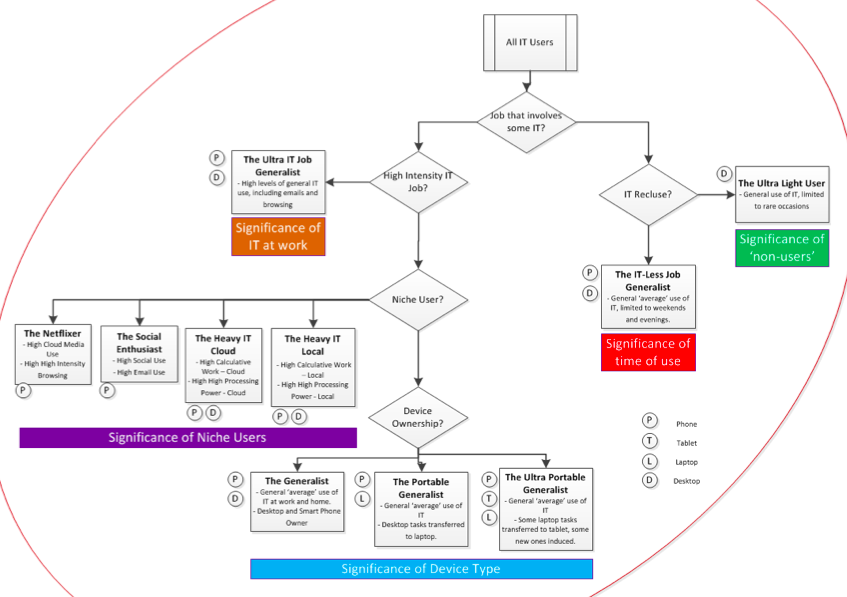
\includegraphics[width=\textwidth]{images/ukitusers_ownership_signif.png}
\caption{IT Users in UK, Device Ownership, and Significance to this Analysis}
\label{fig:itusersuk} 
\end{figure*}

Our estimations of the relative proportions of each segment can be
seen in Figure~\ref{fig:marketshare}.  Using primary market research
into user behaviour, we decided upon the types of days of use;
typically `average weekend' and `average weekday' for most users. For
each day a timetable of use, to a resolution of 0.5 hour slots, was
specified. These can be seen in supporting information section 1.

\begin{figure}[!ht]
\centering
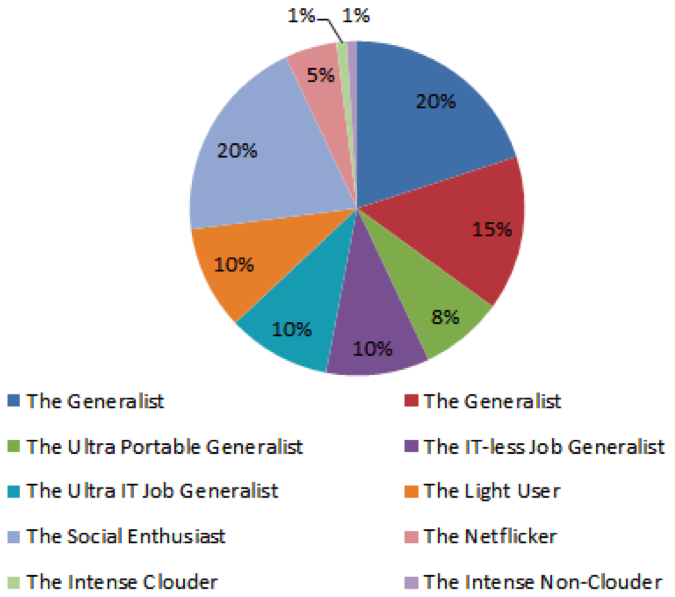
\includegraphics[width=\columnwidth]{images/ukitusers_marketshare.png}
\caption{Assumed Market Share of IT User types in UK}
\label{fig:marketshare} 
\end{figure}


\subsection{Use - Device}

The purpose of this section is to define an average user’s IT use.

\subsubsection{Use Case States}

A device can be used for many different purposes, any one of which we will define as a Use Case.
To identify a suitable selection of use cases, we initially
brainstormed a great number of possible use cases. We then filtered
down the selection to satisfy the following criteria:

{\textbf{Excluding those that show unusual behaviour in the device
    components:}} this excluded gaming, where Graphics Card power can be up to 250\% of
a standard desktop’s power, discussed in the other components section
later.

{\textbf{Including those that are most prevalent:}} this excluded listening to
music and scanning.

{\textbf{Excluding those that are insufficiently different to an idle
    state:}} this excluded background system tasks such as watchdogs and network
updates.

{\textbf{Including those that are necessarily distinct in order to
    comment on the key issues within our scope:}} including cloud and
non-cloud variations of similar tasks.

The final use case selection can be seen in Figure 8.

\subsubsection{Use Case Characteristics}

The purpose of this section is to explore how a device behaves in general under different use cases.

\noindent {\textbf{Component Parts}}

For this analysis we will categorise the power consuming components of
a device into four categories:

\begin{itemize}
\item The CPU - including all integral elements.
\item The Display - inclusive of the power to power the display only.
\item Network Components - any power-consuming component that is used to transfer data in or out of the device.
\item Other Components - inclusive of all power-consuming components
  of the device not covered in the above three categories as well as
  peripherals. Includes RAM, hard drive, motherboard, graphics
  card, sound cards in the first element; printers, scanners and input
  devices in the second.
\end{itemize}

\noindent {\textbf{Characteristics}}

A Use Case has four principle characteristics:

\begin{itemize}
\item CPU Power Factor - the variation of the CPU’s power in a given use case.
\item Display Power Factor - the variation of the Display’s power in a given use case.
\item Other Power Factor - the variation of others in a given use case.
\item Data Flow - the magnitude of data (summation of in and out) flow during a use case.
\end{itemize}

\noindent {\textbf{Use Case States - Power Factors}}

The aforementioned power factors affect the given power use of each
device component, on average, in a given use state. These are
calculated thus:

CPU = CPU Idle power * CPU power factor\\
Other = CPU Idle Power * Other power factor\\
Display = Display average * Display power factor\\

These methodologies are discussed and justified in the following
component sections.


\noindent {\textbf{CPU}}

CPU power use and CPU utilisation does not follow a linear
relation. In practice, the CPU consumes tangible power when idle, and
then increases from this to anything from 2-10 times the idle power at
100\% utilisation.  After primary research, we can observe that
certain types of use case manifest themselves as slight different
tasks on different devices. For example, high intensity browsing, such
as viewing of a video on YouTube will typically be done at a
resolution of the device or lower. As such, the task will require less
processing power on smaller devices. Others will not scale in this
way, for example a word document will be the same size and complexity
of word document regardless of device size.

We theorise that for scalable tasks, the down scaling of task’s
intensity can be approximated as balancing out with the decrease in
processing power for smaller devices. For non-scalable tasks, we
theorise that applying the above approximation to them will be of
little inaccuracy, as such unscalable tasks are typically of such low
processing intensity that the practical utilisation will be only
slightly higher on less powerful CPUs.  These assumptions culminate in
having a `power factor' for a given use case that is common to all
four device types.

As such CPU power use varies with the intensity of task it
undertakes. Through primary research we have ascertained that
instantaneous CPU power use, on modern CPUs, is typically low, <30\%
for most tasks, and that average CPU intensity lower still. By primary
research we have obtained estimations of average CPU powers for all of
the use cases defined. These can be seen in
Figure~\ref{fig:cpuintensity} below. We can see that the majority of
applications use little power above idle, with a few select tasks
actually using the full power of the device. This aligns with other
research in the field of CPU design and use. For a standby mode of any
device, the CPU rests at its idle power.

\begin{figure}[!ht]
\centering
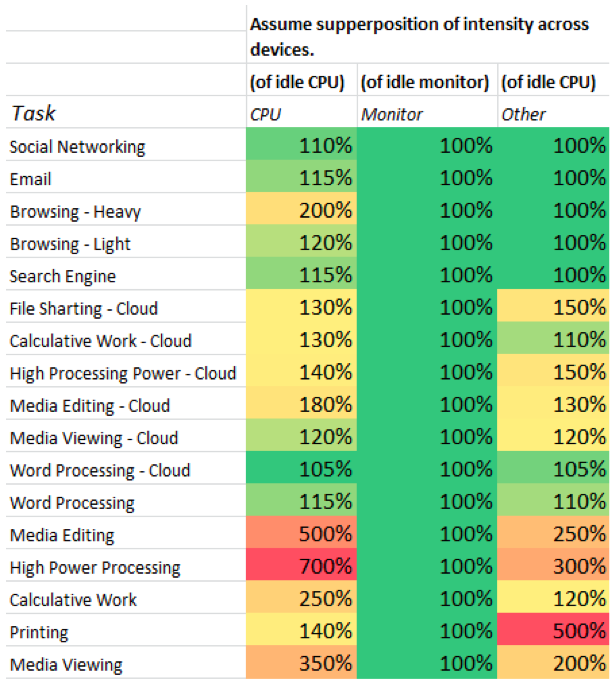
\includegraphics[width=\columnwidth]{images/cpuintensity_usecase.png}
\caption{CPU Intensity by Use Case}
\label{fig:cpuintensity} 
\end{figure}

\noindent {\textbf{Display}}

Research suggests display power is not dependent upon the level of
activity on a screen: changing content does use energy in the
display. Research also suggests that in modern displays, the exact
colour of the content is not related to power consumption. The only
distinct characteristic proven to influence the power consumption is
the brightness setting of the display.

In can be seen that this is typically unrelated to a task. Indeed, it
could be said that individuals may lower the brightness during long
working hours, such as extensive typing, or raise it when the quality
and clarity of the image is crucial, such as when watching a
film. This however, is most probably a matter of personal taste, and
the inter-use-case-brightness-level variation is likely to be less
significant than the individual’s average preferences on brightness.

\noindent {\textbf{Network}}

Network connection power is typically perfectly inelastic to data, and
as such is evaluated as constant for each type, discussed by device in
later sections. As such, no power factors exist for network devices.

\noindent {\textbf{Other}}

The power from the remaining components is difficult to estimate
without considering the power uses of individual devices. As such,
these can be inferred from the remaining observed power use of a given
device when network and CPU powers have been taken out, as determined
in later sections.

With regards to power factors, there are two elements that exist:

{\textbf{A) The use of peripherals to service a task:}} the inclusion of extra
devices to facilitate an end, such as printers, scanners and such. The
power impact of such devices is given by their independent power
ratings.

{\textbf{B) The power of internal components in relation to task
    intensity:}} research suggests most other components scale very little with task
intensity, and change their power more based on specific nuances - for
example the HD with file sharing, the graphics card with media
viewing. As such, this is considered to be a smaller influence than
the peripherals

% For each task, the other power factor will be estimated based on the
% above factors. The other power factor will then be multiplied by the
% device’s idle CPU power. With the assumption of equal intensity, while
% this will hold true for B, it will also result in some inaccuracies in
% A, implying the peripherals will scale with the device’s CPU. In
% mitigation, some of these situations will never be observed, such as
% printing from a phone. Others will, such as printing from a laptop,
% but we will note these inaccuracies, which we deem to be small, as a
% point of further improvement.


\subsubsection{Use -- Supporting Infrastructure}

The energy associated with data flow which is consumed by supporting
infrastructure is outlined in more detail in supporting information
section 4, and summarised in Table 7 below.

\subsubsection{National Grid Electricity}

The final data requirement for this analysis is the carbon intensity
of the energy used by the individual and their IT-related
activities. As previously mentioned, this report aims to assess the
chronological impact of the IT use, and this has been achieved using
primary data collected from the realtimecarbon project
(realtimecarbon.org), rather than a static average value for the
greenhouse gas impact of grid electricity.

The figure commonly quoted for UK national grid carbon intensity is
445.48g CO$_2$ (Carbon Trust) per unit of energy (1kWh), however in
reality this figure changes over the course of the day, and over a
longer time period, depending on what energy sources are being used
and their relative contributions to the current grid mix. This is
summarised in Table 8 below, and data and discussion of the analysis
is outlined in supporting information section 4.


\section{Results}

\subsection{Chronological View}

Figure~\ref{fig:generalist_weekday} demonstrates the energy use, by
the device that causes it, and then by component, for The Generalist’s
`Average Weekday'. Point A shows the minuscule standby power
(erroneously including the screen being on) of the phone
overnight. Point B highlights the increase in device power of
printing. Point C demonstrates the only perceptible time the phone’s
energy consumption is tangible, during heavy browsing. Point D
demonstrates the deactivation of the work computer as the user travels
home; Point E shows the activation of the home desktop upon arrival,
entering standby mode. Point F shows the increase in device power due
to a small period of media viewing; shortly before this we see the
only tangible power consumption of WAN and Servers, during the high
data task of Heaving Browsing.  Immediately, we can observe that in
almost all situations, the phone’s power is imperceptibly small
compared to the desktop power. Secondly, we can observe that idle
computer power is a significant point of wastage.

\begin{figure}[!htp]
\centering
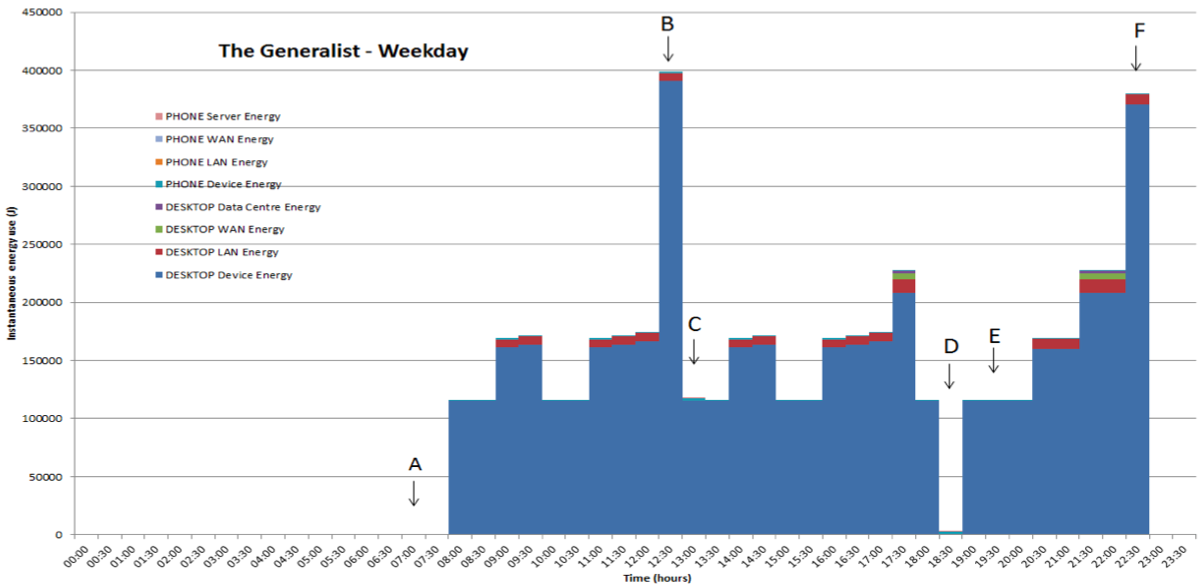
\includegraphics[width=\columnwidth]{images/generalist_weekday.png}
\caption{Energy Use by Device and Component}
\label{fig:generalist_weekday} 
\end{figure}

\subsection{By User}

Figure~\ref{fig:energyuse_co2e_overyearbyuser} demonstrates the
energy, in use CO$_2$e and embodied CO$_2$e by user type.  Immediately, we
can observe that there is a substantial variation in the environmental
impact by the type of user. We will discuss the significance of this
in the conclusion.

\begin{figure}[!htp]
\centering
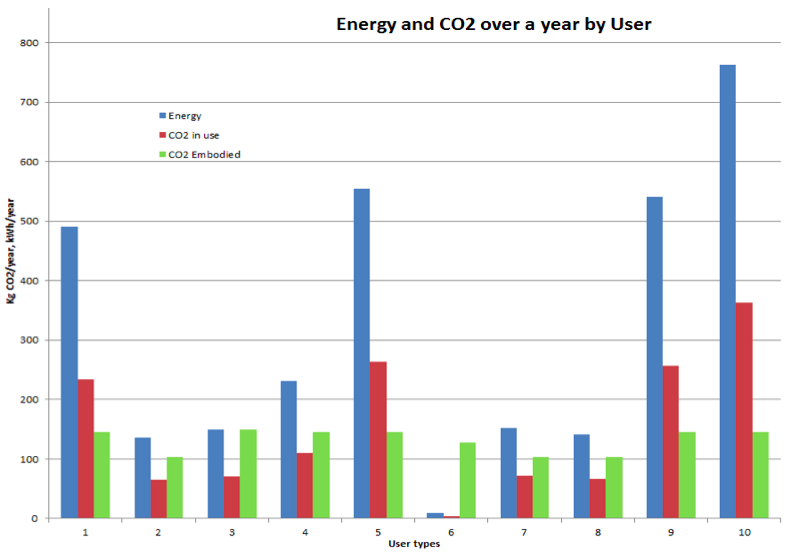
\includegraphics[width=\columnwidth]{images/energyuse_co2e_overyearbyuser.png}
\caption{Comparison of Energy Use and CO$_2$e for Users}
\label{fig:energyuse_co2e_overyearbyuser} 
\end{figure}

\subsection{By Infrastructure}

Figure~\ref{fig:energyusecomparison} demonstrates the energy use by
infrastructure type.  Immediately we can observe that the device
dominates the power use across all user types covered. LAN appears an
order of magnitude smaller, WAN and Server an order of magnitude
smaller again, and roughly equal to each other. Secondarily, we can
observe that the exact proportions of all four energy types vary
considerably depending on the user type.

\begin{figure}[!htp]
\centering
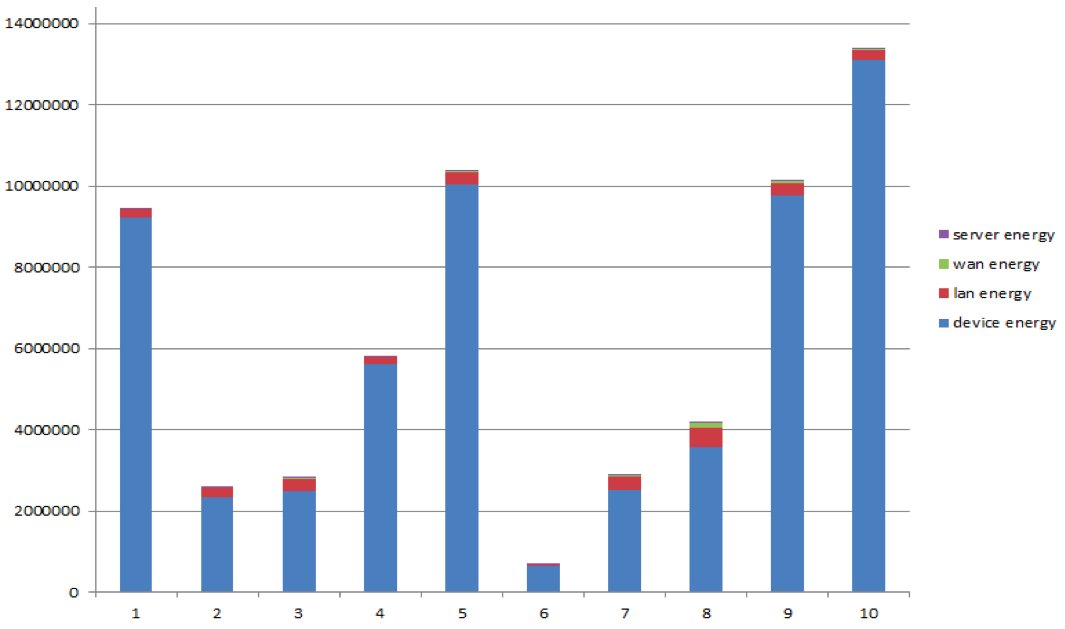
\includegraphics[width=\columnwidth]{images/energyuse_comparison.png}
\caption{Comparison of Energy Use of Device and Infrastructure}
\label{fig:energyusecomparison} 
\end{figure}

\subsection{Estimation of IT Impact of one average UK individual in
  one year}

Final calculations show that, when prototypical days and user type
distribution is taken into account, the impact of one average UK
individual in one year is:

Total energy use: 259kWh\\
Total in use carbon: 123.7kg\\
Total embodied carbon: 127.1kg\\

The tabulated values of energy and carbon by each prototypical day for
each user, which have been used to produce this calculation, can be
seen in supporting information section x?.

% \subsection{Validation}

% The approximate total annual energy consumption (kWh) for devices/user
% seem reasonable when compared to EnergyStar TEC and sust-it.net
% analysis. The latter states:

% - Desktop: approx 50kWh - 200kWh per year, \pounds 6-\pounds 28\\
% Laptop: approx 6kWh-55kWh, \pounds 1-\pounds 8\\

% Our equivalent cost of \pounds 39 seems a realistic value for the time
% period.  Our slightly higher value can be attributed to the inclusion
% of both wider infrastructure, standby power and the inclusion of
% extreme user groups such as The Intense Clouder and The Intense Non-
% Clouder.


\section{Conclusions}

% \subsection{Significance of Chronological Context}

% To further evaluate the significance of carbon variation we will
% compare two identical situations: the social enthusiast using social
% networking on a 3G phone at different times of the day.

% As Figure~\ref{fig:ghgimpact_times} shows, the grid carbon varies
% within a sufficient proportion of the day’s hours that users are
% active in both the highs and the lows. As such, social networking on
% the commute to work is about 6.7\% more carbon intensive than a
% session shortly before bed.

% \begin{figure}[!ht]
% \centering
% 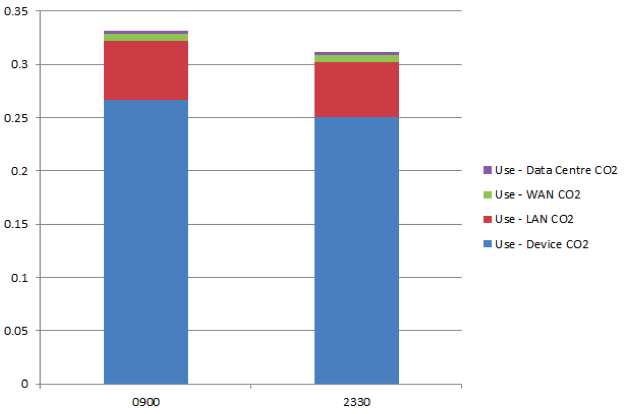
\includegraphics[width=\columnwidth]{images/ghgimpact_times.png}
% \caption{GHG Impact of Identical Action at Different Times}
% \label{fig:ghgimpact_times} 
% \end{figure}

\subsection{Significance of IT at Work}

The benefit of exploring varying user behaviour is the ability to
differentiate domestic and professional IT use. The generalist, the
IT-less generalist and ultra IT generalist all own the same
devices. The IT-less generalist only uses his desktop at home; the
Generalist uses it approximately 40\% of their working hours, the
Ultra IT Generalist approximately 80\%. The varying desktop energy use
over a day can be seen in Figure~\ref{fig:ghgvariation_userworkrelatedit}.

\begin{figure}[!ht]
\centering
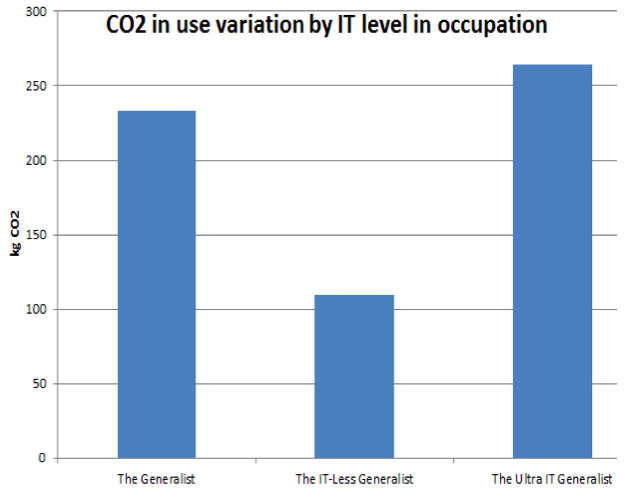
\includegraphics[width=\columnwidth]{images/ghgvariation_userworkrelatedit.png}
\caption{GHG Variation with User Work-Related IT}
\label{fig:ghgvariation_userworkrelatedit} 
\end{figure}

Immediately we can see a non-linear relationship. This can be
explained by the significance of standby power. Having a computer on
at work is the key factor - this immediately adds a large base power
use (Generalist vs IT-Less Generalist), but further use of the
computer makes a much smaller difference (Generalist vs Ultra IT
Generalist).

IT-Less Job Generalist does a little more desktop use at home as a
result and delegates some of the would-be-desktop day time activity
down to a phone, but both are insignificant in comparison.

This highlights the significance of workplace policies to minimise
idle computer time. The energy use of workplace computers left on
overnight is not covered in our LCA and could be hugely significant.

\subsection{Significance of Non-Users}

Figure 14 (Section 5.1.2) shows that the in use CO$_2$ of near-non users
is an order of magnitude smaller than other users. This is not only
driven by low use, but exemplified by the efficiency of which they use
their desktop: by turning it off immediately after use, they accrue no
standby power wastage.

However, even though they are modelled to only own a desktop, the
embodied carbon of it is highly significant and as such they cannot be
neglected as a user group - their total carbon footprint is only 20\%
lower than a Portable Generalist.

Furthermore, despite their efficiency of use, this translates overall
to a heavy impact per hours of use - 1.36kg/hour compared to
0.068kg/hour for The Portable Generalist.

\subsection{Significance of Varying Task Types}

Even though the overall impact is dominated by device energy,
situations exist that span many different proportional makeups. It is
important that these are considered should any of these situations
become particularly popular in the future.

An extreme with very low device power proportion can be seen at the
top of Figure 24, a roughly equal split at the middle, and an extreme
of high device power proportion at the bottom.

Furthermore, the analysis of individual behaviour allows us to
evaluate common perceptions of the environmental impact of given
device uses.

Figure 25 demonstrates the energy use of a Portable Generalist and two
slight niche variations - the Social Enthusiast and Netflicker.

\begin{figure}[!ht]
\centering
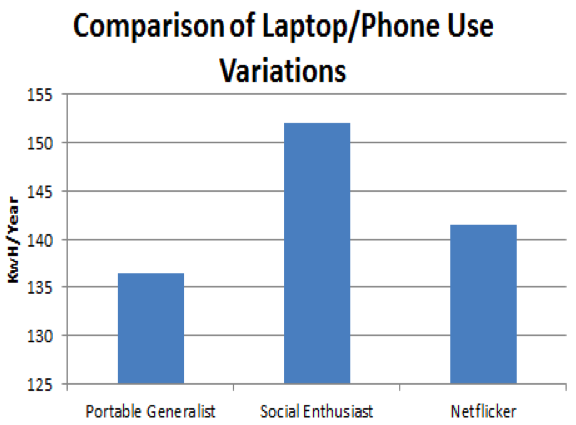
\includegraphics[width=\columnwidth]{images/comparison_users_devices.png}
\caption{Comparison of Different Users and their Devices}
\label{fig:comparison_users_devices.png} 
\end{figure}

Common logic might suggest that streaming a video (using large amounts
of data and increasing CPU load) would be terrible behaviour
environmentally. However, the Social Enthusiast, who typically keeps
his device on longer (particularly on the weekends) to perform a
relatively low intensity task is far worse. Furthermore, the
Netflicker could be considered to be using the concept of cloud
efficiency - streamed videos are typically of a lower codec complexity
than downloaded or DVD/BluRay based video.

\subsection{Significance of Interchangeability of Devices}

Modelling similar behaviour across different devices provides the
ability to comment on how devices can be interchanged and the effects
of this.

% Device interchanging is a voluntary process that has come to light
% with the proliferation of different kinds of devices in the consumer
% market. Where there was once desktops and a few laptop models, there
% is now a myriad of desktop, laptop, tablet and phone devices, and a
% myriad of hybrids not covered in this report. In reality, device
% interchanging is not a simple process, and this was reflected in our
% user types.

\begin{figure}[!ht]
\centering
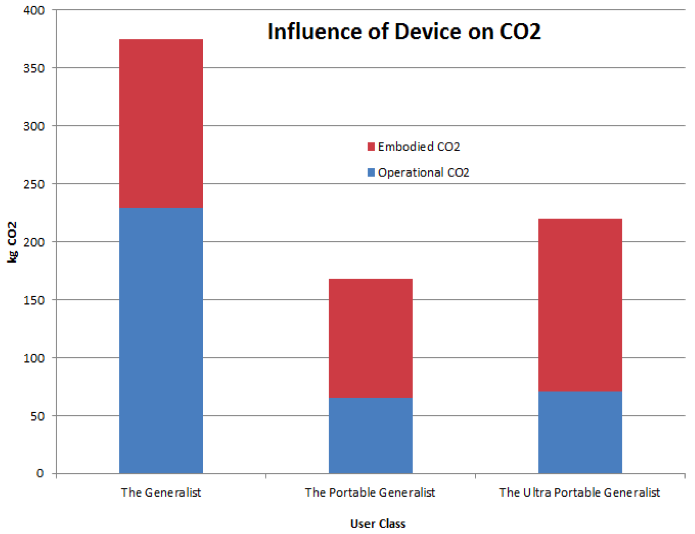
\includegraphics[width=\columnwidth]{images/ghgimpact_devicetypes.png}
\caption{Variation in GHG Impact for Different Device Types}
\label{fig:ghgimpact_devicetype} 
\end{figure}

In our model we assume the Generalist and the Portable Generalist have
identical behaviours - the increase in potability of the device does
not, for the prototypical days covered, induce additional IT
demand. 

% In reality, only a few exceptions to this can be perceived -
% using a laptop in meetings, taking a laptop to a friends house - but
% these are relatively infrequent events in the scale of an individuals
% life. Furthermore, the vast majority of tasks undertaken on a desktop
% can be undertaken on a laptop.

For the Ultra Portable Generalist, we model there being a slight
increase in IT use induced by the inclusion of a tablet. The tablet is
on the individual almost as much as a phone is, and this increase in
portability is somewhat more significant than the desktop-laptop
transition. Some tasks are deemed to be down-scalable to the tablet,
but a lower percentage than those down-scaled the previous
situation. Furthermore, some tasks on the phone are scaled up to the
device, due to the overlap of possession.

Although the energy step up from phone to tablet is much smaller than
the step down from laptop to tablet, the saving here roughly equates
to the sum of the actions scaled up from the phone and the induced
actions. When the greater embodied carbon is then included, we can see
the inclusion of new smaller device has actually resulted in a greater
environmental impact of the Ultra Portable Generalist than the
Portable Generalist.  Crucially, this difference is small compared to
the differences between both of these users and the original,
desktop-based Generalist. It could be logically concluded the extra
carbon for The Ultra Portable Generalist is a small price to pay for
the extra benefits of a tablet, and certainly preferable to The
Generalist. Indeed, one could theorise that a policy to give away
tablets in return for old desktop computers would, at least in theory,
be highly effective.

Ultimately this is a very complex topic that involves psychological
and market forces and is only lightly touched upon here. From the
theory here, a dream solution appears to make 98\% of individuals use
only a phone; our knowledge of reality knows this is a ridiculously
impractical suggestion. Crucially though, the relationship between
devices, behaviour and carbon is highly significant and in the opinion
of this paper, warrants further research.

\subsection{Relative Significance of Device and Supporting
  Infrastructure}

Figure X summarises what is already immediately apparent from Section
5.1.3 and what is perhaps the strongest trend in all of our findings:
device energy dominates. The logical progression of this is the CPU
intensity of a task is a far better indicator of its environmental
impact, at least in most situations, than the data flow.  If accurate,
this suggests that efforts to reduce server and LAN power would be
better spent on reducing device energy.

\section{Recommendations}

\subsection{Personal}

\subsubsection{Downscaling}

As the above results show, different use characteristics produce wide
variation in the consumed energy and CO$_2$ production. The most apparent
variation is in the contrast between desktop use and smartphone
use. This gives credence to to recommendation to use a smartphone over
a desktop where possible, especially for low power tasks such as
internet browsing. This raises practical issues, so a significant
benefit can also be made by the transition from desktop to laptop with
much more ease. With the exception of the 2\% of Intense Clouders and
Intense Non-Clouders, the vast majority of users’ tasks should be able
to transition flawlessly (at least in the technical sense).

% Light users, whose embodied dominates their overall carbon impact,
% could make a substantial reduction by using a laptop over a
% desktop. Furthermore, these individuals could purchase a smart phone,
% even if for their own entertainment, and make negligible difference to
% their overall impact.

In a commercial context, the operating costs of an office run off
laptops as opposed to desktops would be significant, and also provide
more flexibility.

\subsubsection{Re-scheduling}

The results also shows a significant variation in the CO$_2$ produced and
the time of day it is produced. It could be suggested that users carry
out certain activities at particular times to make the most of the CO$_2$
per energy constant at that time but in practice this may not be
suitable for the majority of users, and the benefits may not out-weigh
the hassle.

However, if the highest device energy users - The Intense Clouders and
Intense Non-Clouders - have any flexibility as to when they are able
to undertake their high power processing, careful monitoring of the
live carbon value could result in as much as a 45\% reduction in its
carbon if done at a low point rather than a high point.

These user types also have the highest proportion of device
energy. That is to say, those with high energy use over a year
typically pay a larger share of that (on the assumption WAN and
Servers are not paid for by the user directly). As such, if
carbon-based taxing or demand-based pricing, as has been suggested,
becomes a reality, this time consideration will make economic as well
as environmental sense.

\subsection{Commercial}

\subsubsection{No Standby Policy}

As highlighted throughout, on a work day, considerable power is wasted
through idle desktops. Screen savers could be an easy quick win for
the effort setting them would, but are unlikely to reduce the overall
wastage by more than 30\%.

Suggesting individuals turn off their computers whenever they are not
directly using them is likely to be completely impractical in the
workplace. However, turning them off outside working hours could
result in a substantial saving, albeit not modelled here. Some
pioneering companies operate network protocols that attempt to shut
down the computer, unless aborted by the user, at the end of working
hours.

There is some synergy between this and the downsizing
recommendation. Laptops would not only use less power in general, but
waste far less sitting in idle.

\subsection{Policy}

\subsubsection{Carbon Grid Tax}

Clearly encouraging large users of electricity, as well as to a lesser
degree the average user, out of high-peak times is beneficial for
reducing the environmental impact of IT, but also to the national
grid, to whom grid variation causes immense financial cost.

If electrical providers are unwilling to switch to `smart pricing' -
electrical pricing based on the demand at that time - then perhaps a
carbon tax, charged based on what CO$_2$ intensity the grid is at any one
point, will give an economic incentive for people to change
behaviour. Furthermore, this will both improve the environment, but
also reduce the cost of variability to the National Grid, which is
funded in part by the government.

Consequentially, this will also make de-carbonisation easier (as low
carbon generation is typically baseload (geothermal, nuclear) or
unpredictable (wind, solar)). Another consequential benefit would be
the motivation of the public for the government to reduce the carbon
of the grid and so reduce their carbon tax.

Admittedly, increasing the price of a sensitive topic such as energy
price would be a political challenge, but if pulled off would be
extremely effective.

\subsubsection{High-Power Leisure Device Regulations}

In the same way that car buyers are put off inefficient cars by road
tax, a tax on high power consuming computer components could be the
answer, such as 200W+ graphics cards. While this may be effective, it
would also be hard to in-force, and ethically questionable if other
entertainment products (TVs, Stereos) were not taxed also. Implying
individuals should adjust their leisure time to be more sustainable
has become a decreasingly popular viewpoint.

Labelling however, such as common practice on other products sold in
the EU, could be a reasonable compromise, encouraging consumers to
make the choice themselves. These have been highly effective on
fridges and other white goods.


\subsection{Further Work}

This section will briefly summarise suggestions for model improvements
discussed throughout:

{\textbf{Monitor Brightness:}} as discussed in Data Collection Strategy,
inclusion of the input of the brightness level a user typically sets
their display to will improve display accuracy across all devices, but
specifically small devices.

{\textbf{Specific Devices within categories:}} as discussed throughout,
inclusion of the option to input specific devices will further
increase accuracy across all devices.

{\textbf{Automation of tool:}} to increase accuracy and ease of primary
research, the tool could be translated into an executable program,
which runs in the background, monitoring the task, data and energy
flows. This could also reference live carbon resources at that
instantaneous moment of action, allowing rapid collection of near-
flawless data.

{\textbf{Relationship Between desktop cost and CPU idle power:}} an
alternative method for estimating the idle power of a given desktop
(to accommodate the large variation), may be to assume that the cost
of a desktop (adjusted to today’s value, where purchased
historically), is proportional to the power of the CPU. Anecdotal
evidence suggests this could be a valid relationship and individuals
are more likely to know when they purchased their desktop, and for how
much, than they are the CPU it contains.

{\textbf{Chronological context of embodied carbon:}} if the dimension
of time is important to use CO$_2$, it is logical to assume it influences
the embodied carbon also. As such, it could be suggested that embodied
carbon for a given device will depend upon the grid power used, the
techniques used, the availability of raw materials and so on. As such,
dependant upon when it was made. This will not only be a useful
investigation to see how older and new devices compare on embodied
carbon, but also to evaluate if the embodied carbon (per CO$_2$ of
device) is general increasing or decreasing over time.


%\newpage

% trigger a \newpage just before the given reference
% number - used to balance the columns on the last page
% adjust value as needed - may need to be readjusted if
% the document is modified later
%\IEEEtriggeratref{28}
% The "triggered" command can be changed if desired:
%\IEEEtriggercmd{\enlargethispage{-5in}}

% references section
\bibliographystyle{IEEEtran}
\bibliography{ict4s2015}

% that's all folks
\end{document}


